\documentclass[../../main.tex]{subfiles}
\graphicspath{{\subfix{../../image/}}} % 指定图片目录,后续可以直接使用图片文件名。

% 例如:
% \begin{figure}[H]
% \centering
% \includegraphics[scale=0.4]{图.png}
% \caption{}
% \label{figure:图}
% \end{figure}
% 注意:上述\label{}一定要放在\caption{}之后,否则引用图片序号会只会显示??.

\begin{document}

\section{模}

\begin{definition}[模]
设 \( R \) 是幺环, \( M \) 是 Abel 群, 其运算为加法. 若有 \( R \times M \) 到 \( M \) 的映射: \( (a,x) \to ax (a \in R, x \in M) \), 对 \( \forall a,b \in R, x,y \in M \) 满足
\begin{enumerate}[(1)]
\item \( a(x + y) = ax + ay \);
\item \( (a + b)x = ax + bx \);
\item \( (ab)x = a(bx) \);
\item \( 1 \cdot x = x \),
\end{enumerate}
则称 \( M \) 为 \( R \) 上的一个\textbf{左模}, 或称 \( M \) 是\textbf{左}\(\boldsymbol{R}\)\textbf{模}, \( ax \) 称为 \( a \) 与 \( x \) 的积, 相应地说, \( R \) 与 \( M \) 间有一个乘法.

类似地, 可定义\textbf{右}\(\boldsymbol{R}\)\textbf{模}, 即有映射 \( (x,a) \to xa (a \in R, x \in M) \), 对 \( \forall a,b \in R, x,y \in M \) 满足
\begin{enumerate}[(1)]
\item \( (x + y)a = xa + ya \);
\item \( x(a + b) = xa + xb \);
\item \( x(ab) = (xa)b \);
\item \( x \cdot 1 = x \).
\end{enumerate}

若 \( M \) 既是左 \( R \) 模, 又是右 \( R \) 模且满足
\[
(ax)b = a(xb), \quad \forall a,b \in R, \ x \in M,
\]
则称 \( M \) 是\(\boldsymbol{R}\)\textbf{双模}, 或称 \( \boldsymbol{R} \) \textbf{模}.
\end{definition}
\begin{remark}
假设 \( R \) 交换环且 \( M \) 是左或右 \( R \) 模, 又对 \( a \in R, x \in M \), 令 \( xa = ax \), 则易证 \( M \) 是一个 \( R \) 模, 今后对于交换环 \( R \) 上的模都指这种意义下的模.
\end{remark}

\begin{example}
数域 \( P \) 上的线性空间 \( V \) 就是一个 \( \boldsymbol{P} \) \textbf{模}. 一般地, 域 \( F \) 上的模都称为 \( F \) 上的\textbf{线性空间}.
\end{example}
\begin{proof}

\end{proof}

\begin{example}
设 \( R \) 是幺环, \( R \) 对加法是 Abel 群, 记为 \( R_+ \). 考虑 \( R \times R_+ \) 到 \( R_+ \) 的映射
\[
(r,x) \to rx, \quad r \in R, x \in R_+
\]
及 \( R_+ \times R \) 到 \( R_+ \) 的映射
\[
(x,s) \to xs, \quad x \in R_+, s \in R,
\]
使 \( R_+ \) 变成一个 \( R \) 模, 因而 \( R \) 可看成它自身上的模.
\end{example}
\begin{proof}

\end{proof}

\begin{example}\label{example:抽象代数-例题1.6.4}
设 \( V \) 是数域 \( P \) 上的线性空间, \( \mathcal{A} \) 是 \( V \) 的一个线性变换, 令 \( R = P[\lambda] \) 为 \( P \) 上的一元多项式环, 则 \( R \times V \) 到 \( V \) 的映射 \( (f(\lambda),x) \to f(\mathcal{A})x, f(\lambda) \in R (x \in V) \), 使 \( V \) 成为一个左 \( R \) 模.
\end{example}
\begin{proof}

\end{proof}

\begin{example}
设 \( M \) 是一个 Abel 群, 运算为加法, 则\( \text{End}M \) 为 \( M \) 的自同态环, 并且 \( \text{End}M \times M \) 到 \( M \) 的映射 \( (\eta,x) \to \eta(x) (\eta \in \text{End}M, x \in M) \), 使 \( M \) 成为一个左 \( \text{End}M \) 模.
\end{example}
\begin{proof}

\end{proof}

\begin{theorem}
设$M$是一个$R$模,则
\begin{enumerate}[(1)]
\item  \( \forall a,a_i \in R, x,x_i \in M, 1 \leqslant i \leqslant n \),
\[
a\left( \sum_{i=1}^n x_i \right) = \sum_{i=1}^n ax_i, \quad \left( \sum_{i=1}^n a_i \right) x = \sum_{i=1}^n a_i x.
\]

\item \( \forall a \in R, x \in M \),
\[
a0 = 0a = 0, \quad a(-x) = (-a)x = -ax.
\]
\end{enumerate}
\end{theorem}
\begin{proof}
\begin{enumerate}[(1)]
\item 

\item 
\end{enumerate}
\end{proof}

\begin{definition}
设 \( M \) 是一个 \( R \) 模, \( M \) 的子集 \( N \) 若满足
\begin{enumerate}[(1)]
\item \( N \) 是 \( M \) 的子群;
\item \( \forall a \in R, x \in N \) 有 \( ax \in N \),
\end{enumerate}
则称 \( N \) 为 \( M \) 的一个\textbf{子模}.
显然, \( \{0\} \) 与 \( M \) 都是 \( M \) 的子模, 称为\textbf{平凡子模}.
\end{definition}

\begin{example}
设 \( V \) 是数域 \( P \) 上的线性空间, \( V \) 的子模即 \( V \) 的线性子空间. 一般域 \( F \) 上的线性空间的子模, 也称为 \( V \) 的线性子空间或子空间.
\end{example}
\begin{proof}

\end{proof}

\begin{example}
设 \( M \) 是一个 Abel 群, 其运算为加法. 映射
\[
(m,x) \to mx, \quad m \in \mathbf{Z}, x \in M,
\]
使 \( M \) 变成一个 \( \boldsymbol{Z} \) \textbf{模}.并且 \( M \) 的子集 \( N \) 为子模当且仅当 \( N \) 为 \( M \) 的子群.
\end{example}
\begin{proof}

\end{proof}

\begin{example}
设 \( R \) 是一个幺环, \( R \) 可看成左 \( R \) 模、右 \( R \) 模或 \( R \) 模. 又设 \( N \) 是 \( R \) 的子集, 则 \( N \) 是左 \( R \) 模 (或右 \( R \) 模、\( R \) 模) \( R \) 的子模当且仅当 \( N \) 是 \( R \) 的左理想 (或右理想、理想).
\end{example}
\begin{proof}

\end{proof}

\begin{example}
设 \( V \) 是数域 \( P \) 上的线性空间, \( \mathcal{A} \) 是 \( V \) 上的一个线性变换. 在\refthe{example:抽象代数-例题1.6.4}中, 从 \( \mathcal{A} \) 出发定义了 \( P[\lambda] \) 模 \( V \)、\( V \) 的子集 \( V_1 \) 是 \( P[\lambda] \) 子模当且仅当 \( V_1 \) 是 \( \mathcal{A} \) 的不变子空间.
\end{example}
\begin{proof}

\end{proof}

\begin{theorem}
设$M$是一个$R$模,则
\begin{enumerate}[(1)]
\item \( M \) 中任意多个子模之交仍为子模.

\item \( M \) 中有限多个子模 \( N_1, N_2, \cdots, N_r \) 之和
\[
N_1 + N_2 + \cdots + N_r = \{x_1 + x_2 + \cdots + x_r | x_i \in N_i\}
\]
仍为 \( M \) 的子模.

\item 设 \( S \) 为 \( M \) 的子集, 则 \( M \) 中包含 \( S \) 的最小子模是所有包含 \( S \) 的子模之交, 称为\textbf{由\(\boldsymbol{S}\)生成的子模}. 若 \( S = \{y_1, y_2, \cdots, y_k\} \) 为有限集, 则 \( S \) 生成的子模为
\[
Ry_1 + Ry_2 + \cdots + Ry_k = \left\{ \sum_{i=1}^k a_i y_i \bigg| a_i \in R \right\}.
\]

特别地, 由一个元素 \( x \) 生成的子模 \( Rx \) 称为\textbf{循环子模}. 若 \( M \) 是由一个元素 \( x \) 生成, 即 \( M = Rx \), 则称 \( M \) 为\textbf{循环模}.

循环群就是循环 \( \mathbf{Z} \) 模. 幺环 \( R \) 就是循环 \( R \) 模.
\end{enumerate}
\end{theorem}
\begin{proof}
\begin{enumerate}[(1)]
\item 

\item 

\item 
\end{enumerate}
\end{proof}

\begin{theorem}
设 \( N \) 为 \( R \) 模 \( M \) 的子模.\( \overline{M} = M/N \) 为 \( M \) 对 \( N \) 的商群, 定义 \( R \times \overline{M} \) 到 \( \overline{M} \) 的映射
\[
(a, x + N) \to ax + N, \quad \forall x \in M, a \in R,
\]
则 \( \overline{M} \) 为 \( R \) 模, 称为 \( M \) 对 \( N \) 的\textbf{商模}.
\end{theorem}
\begin{proof}
首先证明上述映射是单值的, 即 \( R \) 中元素 \( \overline{M} \) 中元素所作乘法运算的合理性.

设 \( x_1, x_2 \in M \) 且 \( x_1 + N = x_2 + N \), 于是 \( x_1 - x_2 \in N \), 因而, 由 \( N \) 为子模有 \( a(x_1 - x_2) = ax_1 - ax_2 \in N \), 故 \( ax_1 + N = ax_2 + N \), 即上面映射是单值的.

以下只要验证 \( R \) 模的 4 个定义条件. 这些验证不难.
\end{proof}

\begin{definition}
设 \( M, M' \) 为两个 \( R \) 模. 如果 \( M \) 到 \( M' \) 的映射 \( \eta \) 满足 \( \forall a \in R, x, y \in M \) 有
\begin{enumerate}[(1)]
\item \( \eta(x + y) = \eta(x) + \eta(y) \), 即 \( \eta \) 是群同态;
\item \( \eta(ax) = a\eta(x) \),
\end{enumerate}
则称 \( \eta \) 为 \( M \) 到 \( M' \) 的一个\textbf{模同态}或\(\boldsymbol{R}\)\textbf{同态}.

若 \( \eta \) 还是满映射, 则称 \( \eta \) 为\textbf{满同态}, 此时称 \( M \) 与 \( M' \) 同态.

\( \eta \) 若还是一一对应, 则称 \( \eta \) 为\textbf{模同构}或\(\boldsymbol{R}\)\textbf{同构}, 此时称 \( M \) 与 \( M' \) 同构, 记为 \( M \cong M' \).
\end{definition}
\begin{remark}
模同态的定义知\textbf{模同态必为群同态.}
\end{remark}

\begin{example}\label{example:抽象代数-例题1.6.10}
设 \( M, M' \) 是两个 Abel 群, \( \eta \) 是 \( M \) 到 \( M' \) 的群同态, 则 \( \eta \) 也是 \( \mathbf{Z} \) 模 \( M \) 到 \( \mathbf{Z} \) 模 \( M' \) 的模同态; 若 \( \eta \) 为群同构, 则 \( \eta \) 也是模同构.
\end{example}
\begin{proof}

\end{proof}

\begin{example}
设 \( N \) 是 \( R \) 模 \( M \) 的子模, \( \pi \) 是 \( M \) 到商模 \( \overline{M} = M/N \) 的自然映射, 即 \( \pi(x) = x + N (\forall x \in M) \). 已知 \( \pi \) 是群同态, 又对 \( \forall a \in R, x \in M \) 有 \( \pi(ax) = ax + N = a(x + N) = a\pi(x) \), 故 \( \pi \) 也是模同态, 称 \( \pi \) 是 \( M \) 到 \( M/N \) 上的自然同态.
\end{example}
\begin{proof}

\end{proof}

\begin{example}
假设 \( V \) 是域 \( F \) 上的线性空间. \( V \) 到自身的模同态 \( \mathcal{A} \), 称为 \( V \) 的线性变换. 显然, 当 \( F \) 为数域时, \( \mathcal{A} \) 就是线性代数中讲的线性空间的线性变换.
\end{example}
\begin{proof}

\end{proof}

\begin{theorem}
设$M$是一个$R$模,
\begin{enumerate}
\item 设 \( \eta \) 是 \( M \) 到 \( M' \) 的 \( R \) 同态, 则 \( \eta(M) \) 是 \( M' \) 的子模且 \( \eta \) 是 \( M \) 到 \( \eta(M) \) 上的同态.

\item 设 \( \eta \) 是 \( R \) 模 \( M \) 到 \( R \) 模 \( M' \) 的同态, \( \eta' \) 是 \( R \) 模 \( M' \) 到 \( R \) 模 \( M'' \) 的同态, 则 \( \eta'\eta \) 是 \( M \) 到 \( M'' \) 的模同态 (\reffig{figure:交换图3}).

\item \( R \) 模之间的同构关系是等价关系.
\end{enumerate}
\end{theorem}
\begin{figure}[H]
\centering
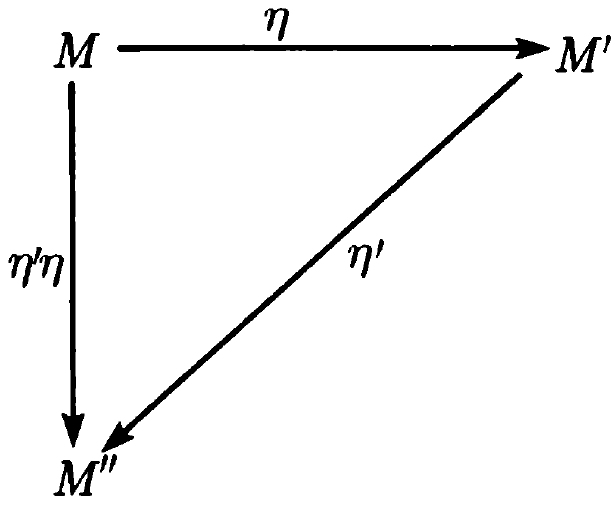
\includegraphics[scale=0.2]{交换图3.png}
\caption{}
\label{figure:交换图3}
\end{figure}
\begin{proof}
\begin{enumerate}
\item 

\item 

\item 
\end{enumerate}
\end{proof}

\begin{definition}
一个 \( R \) 模 \( M \) 到自身的同态称为 \( M \) 的 \( R \) 自同态, 简称\textbf{自同态}. \( R \) 模 \( M \) 的 \( R \) 自同态的集合记为 \( \text{End}_R M \). 

以 \( \text{End}M \) 表示 Abel 群 \( M \) 的所有群自同态的集合.
\end{definition}
\begin{remark}
由模同态的定义知模同态必为群同态, 故有 \( \text{End}_R M \subseteq \text{End}M \). 另一方面, 可以验证在 \( \text{End}M \) 中可定义加法与乘法使 \( \text{End}M \) 是一个环. 
\end{remark}

\begin{theorem}\label{theorem:抽象代数-定理 1.6.2}
设 \( M \) 是一个 \( R \) 模, 则 \( M \) 的 \( R \) 自同态的集合 \( \text{End}_R M \) 是 Abel 群 \( M \) 的自同态环 \( \text{End}M \) 的子环. \( \text{End}_R M \) 称为 \( R \) 模 \( M \) 的\textbf{模自同态环}.
\end{theorem}
\begin{proof}
显然, \( \text{id}_M \in \text{End}_R M \), 故 \( \text{End}_R M \neq \varnothing \), 又若 \( \eta_1, \eta_2 \in \text{End}_R M \), \( x, y \in M \), \( a \in R \), 则有
\[
(\eta_1 - \eta_2)(x + y) = \eta_1(x + y) - \eta_2(x + y) = (\eta_1 - \eta_2)(x) + (\eta_1 - \eta_2)(y),
\]
可知 \( \eta_1 - \eta_2 \in \text{End}_R M \), 故 \( \text{End}_R M \) 对加法成群. 又由同态性质知 \( \eta_1\eta_2 \in \text{End}_R M \), 由此可知 \( \text{End}_R M \) 是 \( \text{End}M \) 的子环.
\end{proof}

\begin{example}
设 \( M \) 为 Abel 群, 于是 \( M \) 为 \( \mathbf{Z} \) 模. 则由\refexa{example:抽象代数-例题1.6.10}知 \( \text{End}_\mathbf{Z} M = \text{End}M \).
\end{example}
\begin{proof}

\end{proof}

\begin{example}
设 \( R \) 是一个幺环, 则 \( R \) 作为左 \( R \) 模有\( \text{End}_R R = R_r \).
\end{example}
\begin{remark}
设 \( M \) 是一个左 \( R \) 模, 一般把 \( M \) 的模自同态环记为 \( _R\text{End}M \). 若 \( M \) 是右 \( R \) 模, 则将 \( M \) 的模自同态环记为 \( \text{End}_R M \). 交换幺环上的模, 可自然地看成双模, 故这时没必要区分这两种记号, 统一地以 \( \text{End}_R M \) 表示.
\end{remark}
\begin{proof}
\( \forall a \in R \), 可定义 \( a \) 的右乘变换 \( a_r \) 为 \( a_r(x) = xa (\forall x \in R) \). 显然, 对 \( \forall x, y, a, b \in R \) 有 \( a_r(x + y) = a_r(x) + a_r(y) \), \( a_r(bx) = bxa = ba_r(x) \), 故 \( a_r \in \text{End}_R R \). 令 \( R_r = \{a_r|a \in R\} \), 即有 \( R_r \subseteq \text{End}_R R \). 现设 \( \eta \in \text{End}_R R \), \( \eta(1) = a \), 于是 \( \eta(x) = \eta(x \cdot 1) = x\eta(1) = xa = a_r(x) \), 即 \( \eta = a_r \). 故 \( \eta \in R_r \), 这样就证明了幺环 \( R \) 作为左 \( R \) 模有\( \text{End}_R R = R_r \).
\end{proof}




























\end{document}